To complete mostt of home serving tasks, our robot consists of three major parts: chassis based on Mecanum wheel, Ball screw Actuator and robot arm including hand. Tinker is about 150cm high. 
\subsubsection{Chassis}
Tinker can move in any direction easily owing to the Mecanum chassis. The chassis consists of 4 separated Mecanum wheel systems, each of which consists of a Mecanum wheel, a brushless DC motor (50W24V), a worm gear box and a brush-less DC motor driver. The PC sends control message to the ZYNQ to command the chassis to move as planed based on ROS. The chassis has a size of 800mm*500mm*200mm.
\begin{figure}[H]
    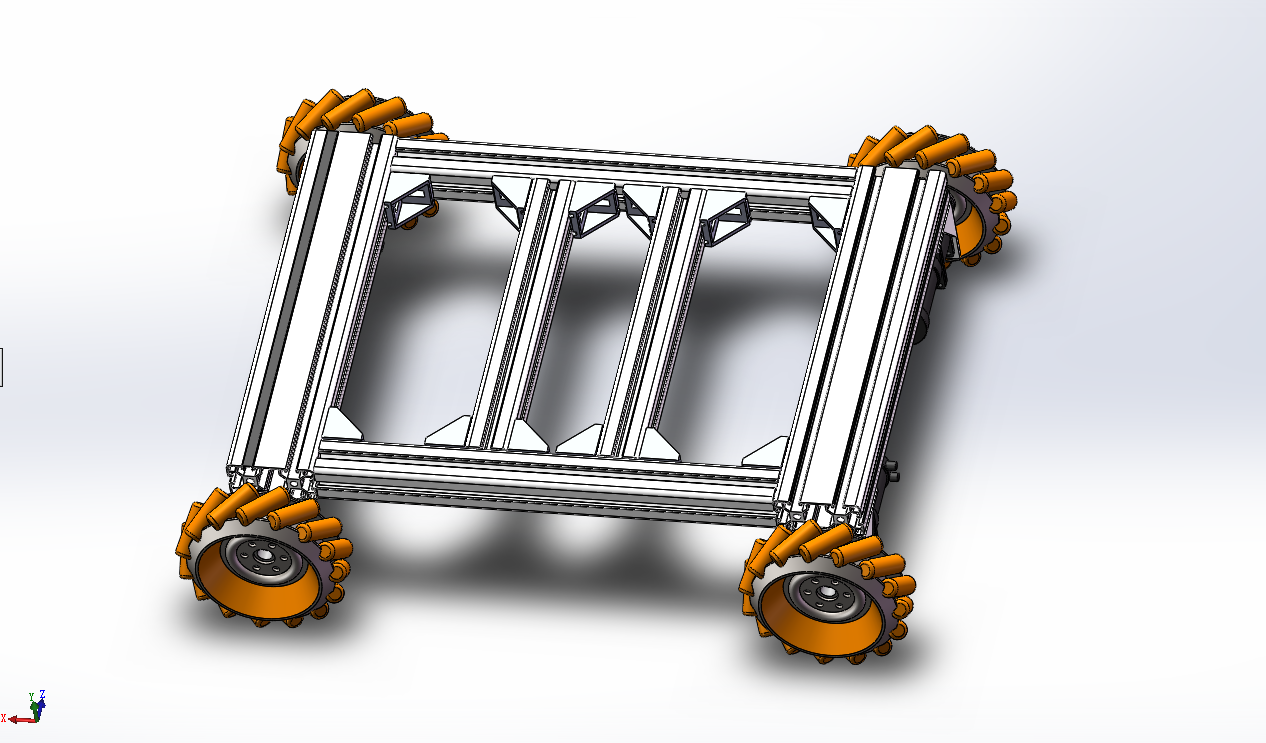
\includegraphics[scale=0.5]{base.jpg}
    \caption{chassis}
\end{figure}

\subsubsection{Robot arm and hand}
The robot arm is the most major part of the mobile robot, used to grasp objects. The complete arm consists of a 3-axis cascade robot arm and a 2-axis robot hand. The 3-axis arm consists of 2 bent joints and a rotate joint; the 2-axis hand consists of a rotate joint which controls the posture and a joint which achieves grasping objects. We use 24V geared DC motor for the arm and MX-64R (Robotis series) as the steering engines for the hand. The maximum length of the arm is about 800mm and it can grasp a 1000g object at maximum length, which is enough in most situations. 
\begin{figure}[H]
    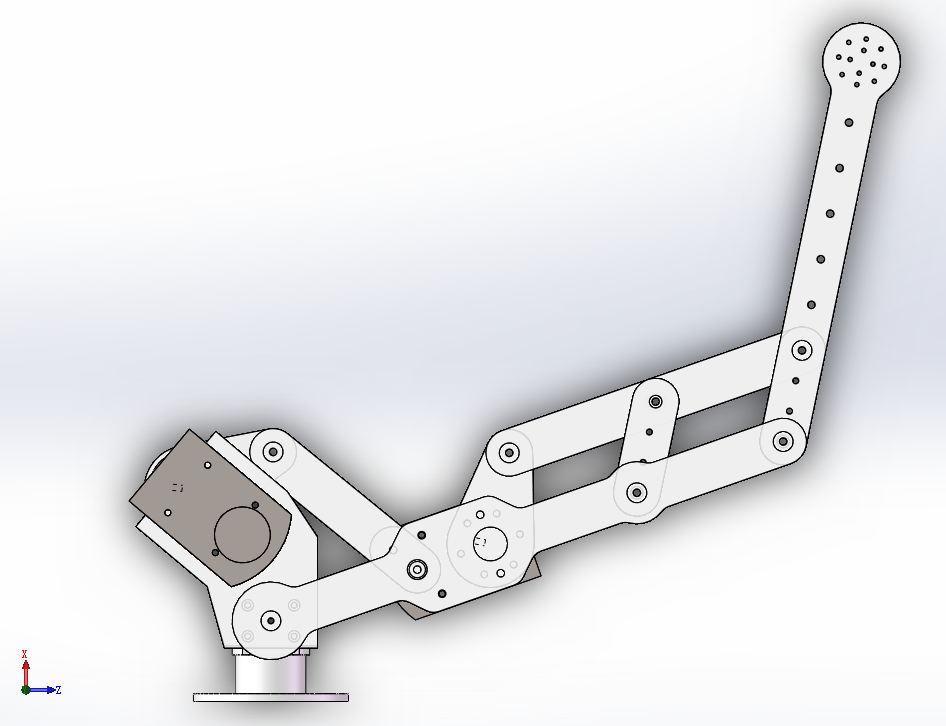
\includegraphics[scale=0.5]{arm.jpg}
    \caption{chassis}
\end{figure}

\subsubsection{Ball screw Actuator}
The bottom of the robot arm is fixed on the Ball screw Actuator so that the arm can be raised or lowered freely, quickly and smoothly. The lift platform enables the robot to manipulate objects of various height. Besides, it provides more workspace.


